%Plantilla adaptada por Luis Chamba-Eras, mayo del 2020.
\documentclass[hyperref={pdfpagelabels=false}]{beamer}
% la Hyperref opci\'on hyperref={pdfpagelabels=false} evita la advertencia :
% Package hyperref Warning: Option `pdfpagelabels' is turned off
% (hyperref)                because \thepage is undefined. 
% Hyperref stopped early 
%
\usepackage[spanish]{babel}
%\useoutertheme{infolines}
\usepackage{lmodern}
\usepackage[ansinew]{inputenc}
\usepackage{color}
%\usepackage[usenames]{color}
%\usepackage[utf8]{inputenc}
% elimina las siguientes advertencias:
% LaTeX Font Warning: Font shape `OT1/cmss/m/n' in size <4> not available
% (Font)              size <5> substituted on input line 22.
% LaTeX Font Warning: Size substitutions with differences
% (Font)              up to 1.0pt have occurred.
%

% cuando  \titel{$B!D(B} \author{$B!D(B} posicina desp\'ues \begin{document} ,
% aparece eso  advertencia: :
% Package hyperref Warning: Option `pdfauthor' has already been used,
% (hyperref) ... 
% Por tanto posicina lo antes de  \begin{document}
\usepackage{amsmath,amssymb,amsthm}
\usepackage{subfigure}
\usepackage{multirow}
\usepackage{epic}
\usepackage{tikz,pgfplots}
\usetikzlibrary{snakes}
\usetikzlibrary{plotmarks}
\usepackage{array}
\usepackage{ragged2e}
\usepackage{graphicx}
\usepackage{fancyhdr}
\usepackage{url}
\usepackage{hyperref}
\usepackage{multicol}
%\useoutertheme{tree}
\usepackage[none]{hyphenat}
\justifying



\mode<presentation>{
	\usetheme{Warsaw}
	\useoutertheme{shadow}
	\usecolortheme{seagull}%dove, seagull
%	\useoutertheme{footline}
	\beamertemplatenavigationsymbolsempty
}

%\setbeamertemplate{background canvas}{\includegraphics[width=\paperwidth,height=\paperheight]{nombre_del_fondo.jp}}

\usebackgroundtemplate{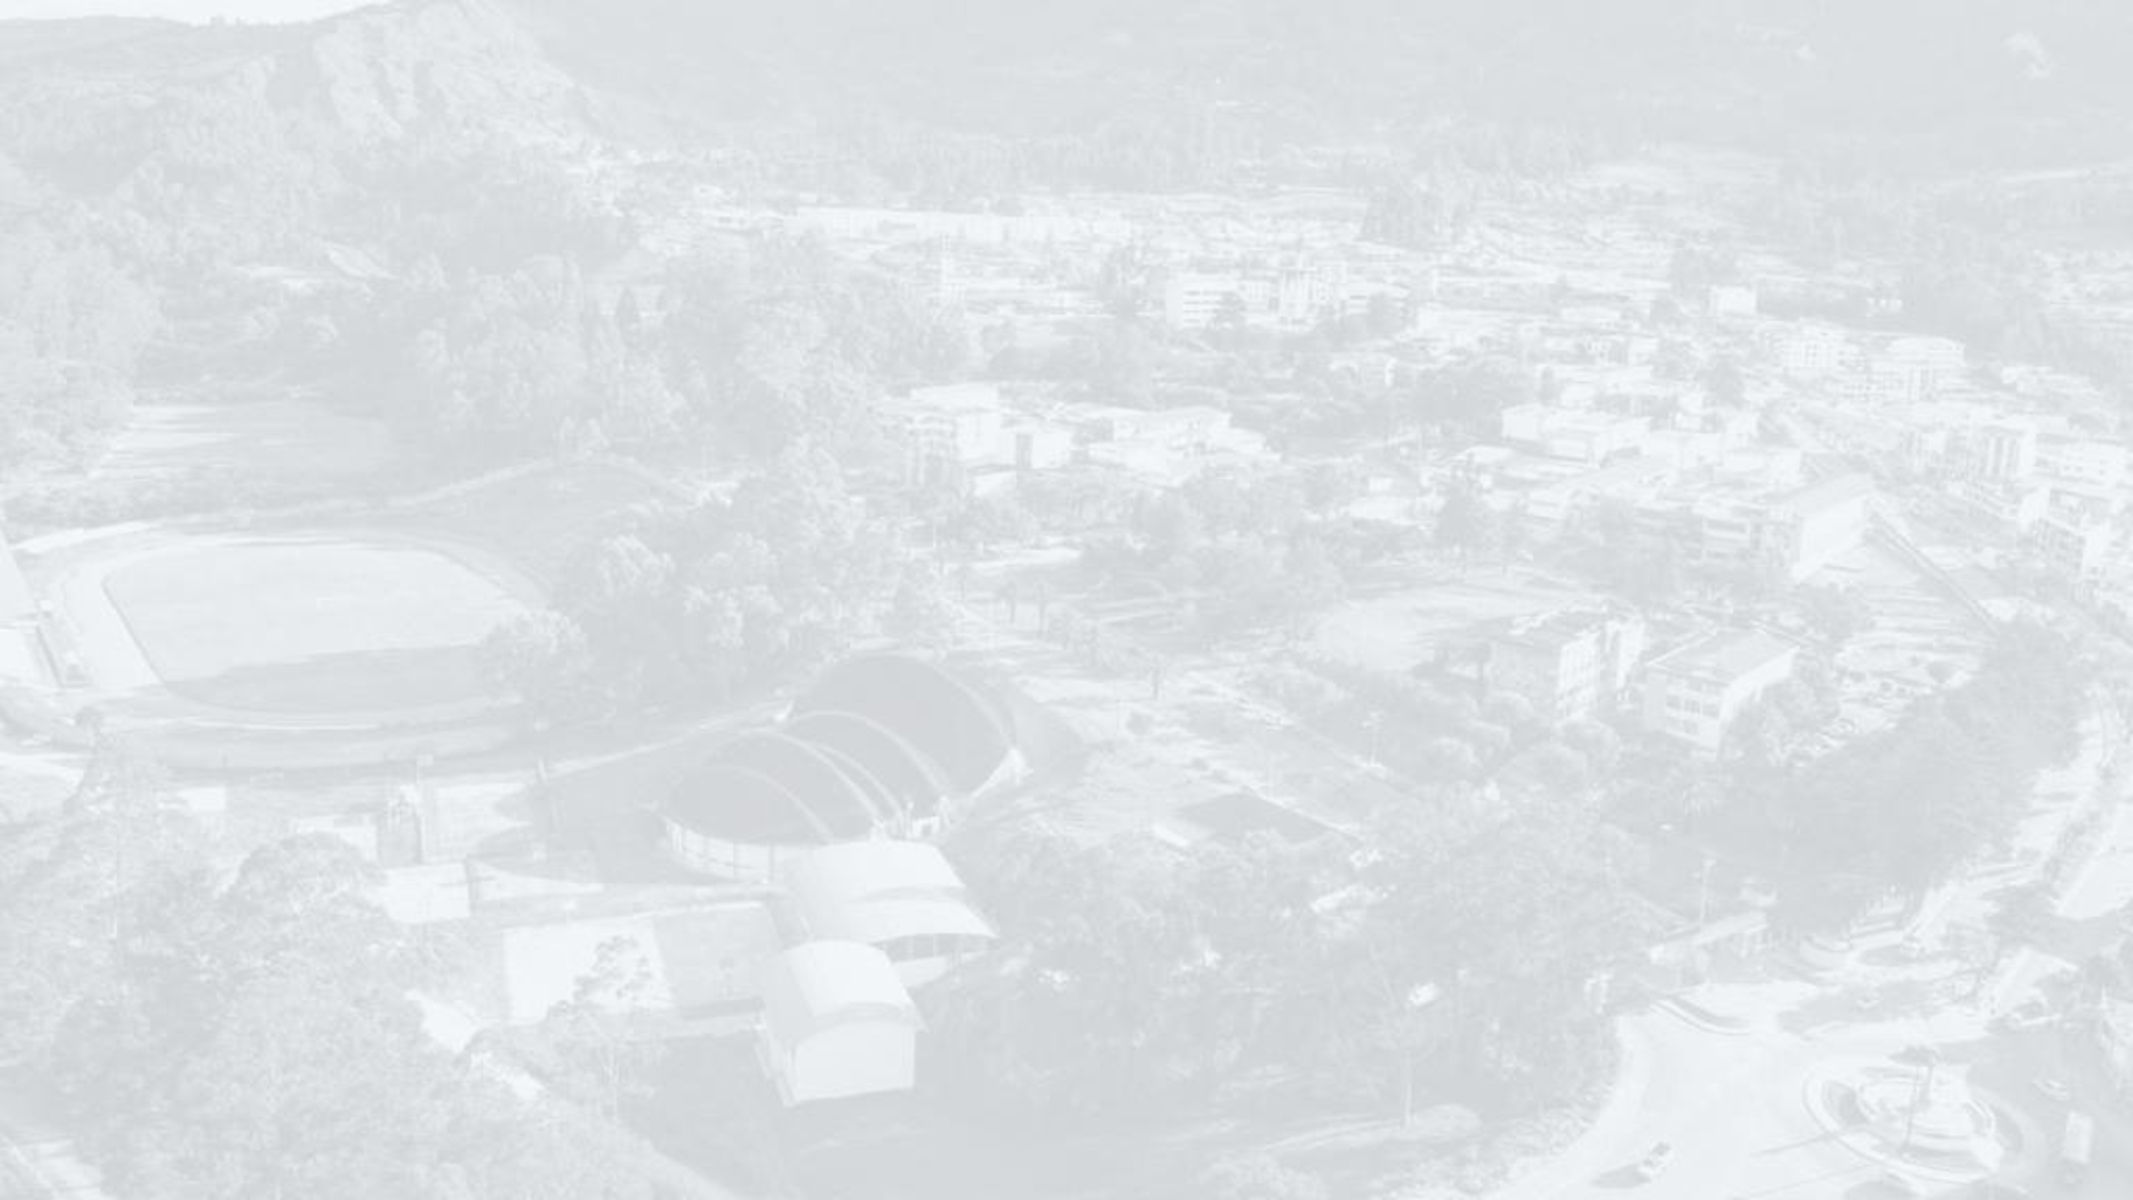
\includegraphics[width= \paperwidth, height=\paperheight]{logos/FondoFinalBlancoUNL.pdf}}
%\addtobeamertemplate{navigation symbols}{}{%
%	\usebeamerfont{footline}%
%	\usebeamercolor[fg]{footline}%
%	\hspace{1em}%
%	\insertframenumber/\inserttotalframenumber
%}

%Eliminar la barra de navegaci�n en la parte inferior derecha de la transparencia.
%\setbeamertemplate{navigation symbols}{}
%\setbeamertemplate{footline}{frame number}
\pgfdeclareimage[height=0.65cm]{unl-logo}{logos/logogris.pdf}
\logo{\pgfuseimage{unl-logo}}

\title[@lachamba - GITIC - GaLan - Tepuy R+D]{Transparencias en LaTeX, versi�n 1.0}   
\author[Luis Chamba-Eras]{Luis Chamba-Eras}

\institute[UNL]
{	
	Universidad Nacional de Loja\\
	Facultad de la Energ�a, las Industrias y los Recursos Naturales No Renovables\\
	Carrera de Ingenier�a en Sistemas/Computaci�n\\
	GITIC, GaLan, Tepuy R+D\\
	Red Loja Investiga, Red Acad�mica SINERGIA
	\and
	Loja, Ecuador
} 
\date{Mayo, 2020} 


% Adicional intercala package{beamerthemeshadow} 
\usepackage{beamerthemeshadow}

\AtBeginSection{ 
	\begin{frame} 
	\frametitle{Agenda}
	\tableofcontents[currentsection]
\end{frame}
}

\AtBeginSubsection{ 
\begin{frame}
\frametitle{Agenda}
\tableofcontents[currentsection,currentsubsection]
\end{frame}
}
\pretolerance=9500
\tolerance=9500

%%%%%%%%%%%%%%%%%Cuerpo del beamer%%%%%%%%%%%%%%%%%%%%%%%%%

\begin{document}

\begin{frame}
\titlepage %portada
\end{frame} 
\begin{frame}
\frametitle{Agenda}
\tableofcontents
\end{frame} 

\section{Resultados de aprendizaje}

\begin{frame}
	\frametitle{Objetivo}
	\begin{block}{}
		\begin{itemize}
			\justifying
			\item Orientar al alumnado para ... 
		\end{itemize} 
	\end{block}
\end{frame}
 
\begin{frame}
	\frametitle{Resultados de aprendizaje}
	\begin{block}{Al finalizar la asignatura se estar� en capacidad de:}
		\begin{enumerate}
			\justifying
			\item Comprender los ...
			\item Dise�ar los ...
			\item Compartir los ...
		\end{enumerate} 
	\end{block}
\end{frame}




\begin{frame}
\frametitle{}
\begin{center}
	\begin{block}{Networking acad�mico}
		\begin{itemize}
			\justifying
			\item Correo electr�nico: \href{mailto:lachamba@unl.edu.ec}{lachamba@unl.edu.ec}
			\item Twitter: \href{https://twitter.com/lachamba}{@lachamba}
			\item URL de la transparencia: \href{https://es.slideshare.net/lachamba}{https://es.slideshare.net/lachamba}
		\end{itemize} 
	\end{block}
\end{center}
\end{frame}

\begin{frame}
	\frametitle{}
	\begin{center}
		{\huge Muchas gracias}
	\end{center} 
\end{frame}
\end{document}